\section{Introducción}
En el caso objeto de estudio de este documento se han planteado la aplicación de los principios 
de \linkeddata para el modelado y explotación de datos e información provenientes de los anuncios de 
licitación públicos. Para ello y como se ha presentado en los anteriores capítulos se ha definido 
un ciclo de vida de datos enlazados que a través de procesos, métodos y tareas suministra una metodología 
de actuación genérica para actuar en este sentido. Como ejemplo de su validez y aplicación se han utilizado 
los datos de los contratos públicos para ejemplificar los procesos de producción, publicación, consumo, validación y 
actualización, ver Figura~\ref{fig:com}. Aunque ciertas tareas se apoyan en el uso de aplicaciones de terceros como Google Refine o bien 
en la parametrización de bibliotecas ya existentes como Apache Lucene, es necesario suministrar un entorno 
en el cual los resultados de aplicar las tareas puedan ser procesados para implementar algunas de las tareas 
especificadas y así ejemplificar transversalmente el uso de datos enlazados en un determinado dominio. Por ello y 
de acuerdo al análisis y especificación realizado se plantea la necesidad de diseñar los componentes del sistema 
MOLDEAS como paso final para la cobertura en el uso de datos enlazados en el campo de la contratación pública 
electrónica y teniendo presente los siguientes objetivos:

\begin{itemize}
 \item Facilitar y dar soporte a las tareas del ciclo de vida que no pueden ser desarrolladas completamente 
por herramientas externas.
\item Validar los datos generados por otras herramientas.
\item Enriquecer con procesos \textit{ad-hoc} la información y datos de los anuncios de licitación según el modelo 
y especificación fijadas en el Capítulo~\ref{capitulo:metodos-separados}.
\item Implementar un demostrador público de consumo de datos enlazados.
\item Proveer un sistema de búsqueda/recomendación de anuncios de licitación de acuerdo a criterios predefinidos 
por el cliente.
\item Establecer un conjunto de prueba que realice la validación parcial de ciertos procesos apoyándose en tecnología 
pre-existente.
\item Diseñar un sistema extensible y escalable para su futura ampliación.
\end{itemize}

\begin{figure}[h]
\begin{tikzpicture}
  \path[mindmap,concept color=gray,text=white]
    node[concept] {MOLDEAS}
    [clockwise from=0]
    child[concept color=green!50!black] {
      node[concept] {moldeas-api}   
      [clockwise from=-90]
      child [concept color=green!80] { node[concept] {\textbf{Consumo}} }   
    }  
    child[concept color=blue] {
      node[concept] {moldeas-transformer}
      [clockwise from=-90]
      child [concept color=blue!50] { node[concept] {\textbf{Producción}} }
      child [concept color=blue!50] { node[concept] {\textbf{Publicación}} }           
    }
    child[concept color=orange] { node[concept] {moldeas-test} 
      [clockwise from=-90]
      child  [concept color=orange!50] { node[concept] {\textbf{Validación}} }      
    }
    child[concept color=red] { node[concept] {moldeas-common} } ;
   
\end{tikzpicture}
    \caption{Alineación inicial de componentes de MOLDEAS y procesos del Ciclo de Vida de \linkeddata.}
 \label{fig:com}
\end{figure}

Ante estos objetivos de gran calado, teniendo en cuenta el ciclo de vida de datos enlazados definido y las tareas 
especificadas para la información y datos presentes en las licitaciones públicas, cabe especificar el diseño 
de los componentes del sistema MOLDEAS como elemento vertebrador tanto de los procesos como de la información. De esta forma, 
a lo largo de este capítulo se hará una descripción del diseño e implementación realizada en el sistema MOLDEAS haciendo 
especial hincapié en los detalles más relevantes del mismo.
\section{Descripción del Sistema MOLDEAS}
La tarea de análisis de un sistema conlleva la especificación de una serie 
de requisitos que guíen el posterior diseño e implementación del sistema 
\gls{MOLDEAS}. De esta forma, se pueden extraer los siguientes objetivos: 
\begin{itemize}
 \item Analizar e identificar el trabajo relacionado.
 \item Identificar y definir los requisitos asociados a las actividades de investigación, 
innovación y desarrollo a realizar.
 \item Especificar los requisitos de usuario para los distintos componentes
 \item Realimentar los puntos anteriores con los resultados obtenidos.
\end{itemize}

Estos objetivos ya han sido parcialmente cubiertos en los anteriores 
capítulos, en los cuales se ha repasado intensivamente la mayoría de los 
trabajos relacionados y relevantes en el dominio de la contratación 
pública electrónica así como se ha puesto de manifiesto los procesos, 
métodos y tareas a desarrollar dentro del ciclo de vida de datos 
enlazados. Es por ello que este capítulo se centrará en presentar las partes más relevantes y 
destacadas del sistema MOLDEAS y su aplicación en las distintas 
tareas del ciclo de vida así como en el desarrollo del sistema de búsqueda 
de anuncios de licitación. En primer lugar, cabe mostrar un esbozo del 
sistema con una vista funcional del mismo, ver Figura~\ref{fig:functional-overview}, en el cual 
se enclavan los distintos procesos del ciclo de vida y los objetivos generales del sistema: 
producción de datos enlazados de los anuncios de licitación para su posterior 
almacenamiento y publicación a través de un \textit{endpoint} de \gls{SPARQL} y un \linkeddata \textit{frontend} y 
consumo de los datos almacenados para la construcción de servicios de valor añadido como el 
sistema de búsqueda/recomendación de anuncios de licitación. Se ha optado por enfoque 
totalmente práctico en este capítulo de ingeniería con el objetivo de resaltar y documentar la innovación del sistema 
MOLDEAS sin focalizar en metodologías intensivas de ingeniería del \textit{software}.


\begin{figure}[!htb]
\centering
	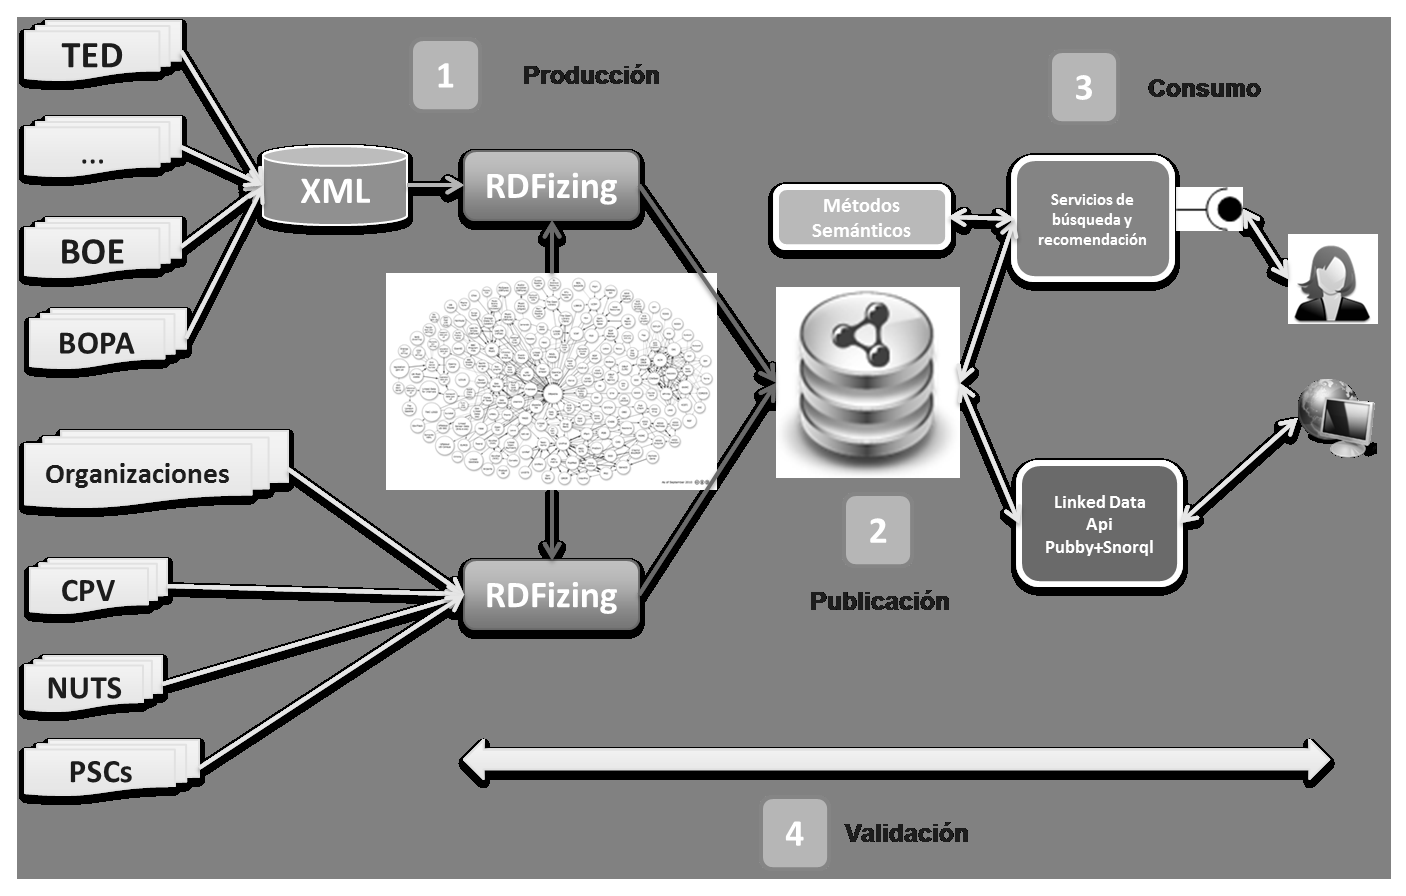
\includegraphics[width=12cm]{images/phd/moldeas/functional-overview}
\caption{Arquitectura funcional del sistema MOLDEAS.}
\label{fig:functional-overview}
\end{figure}

A la vista de la arquitectura funcional propuesta, se ha realizado una aproximación en distintos componentes, 
de acuerdo a sus responsabilidades e interacciones, ver Figura~\ref{fig:moldeas-components}, y con la siguientes 
definiciones:

\begin{description}
 \item [moldeas-common.] Alberga utilidades necesarias a lo largo de todos los procesos del ciclo de vida de datos 
enlazados.
 \item [moldeas-transformer.] Se encarga de dar soporte a la producción de datos enlazados cubriendo las tareas de transformación, 
  enriquecimiento, reconciliación de entidades, etc.  
 \item [moldeas-api.] Se encarga del consumo de los datos enlazados publicados bajo unas 
ciertas características en un \textit{endpoint} de SPARQL y que con la aplicación de varios 
métodos de expansión de consultas es capaz de generar consultas SPARQL cercanas al lenguaje natural 
para la recuperación de los anuncios de licitación.
\item [moldeas-test.] Se encarga de la validación de los datos enlazados y de los métodos de expansión definidos en \texttt{moldeas-api}.
 \item [moldeas-web.] Se encarga de la presentación y consumo de datos enlazados suministrando 
un interfaz gráfico para \texttt{moldeas-api} en el cual el usuario puede seleccionar las 
características de los anuncios de licitación para su posterior búsqueda y 
presentación con diferentes vistas (tabla, mapa, etc.). Además, suministra un interfaz de servicios REST para el acceso 
a los métodos disponibles en \textit{moldeas-api} por lo que cumple una doble función: 1) servir como demostrador 
público para el usuario y 2) ejemplificar las llamadas a \texttt{moldeas-api} desde un punto de vista 
del desarrollador.
\end{description}

\begin{figure}[!htb]
\centering
	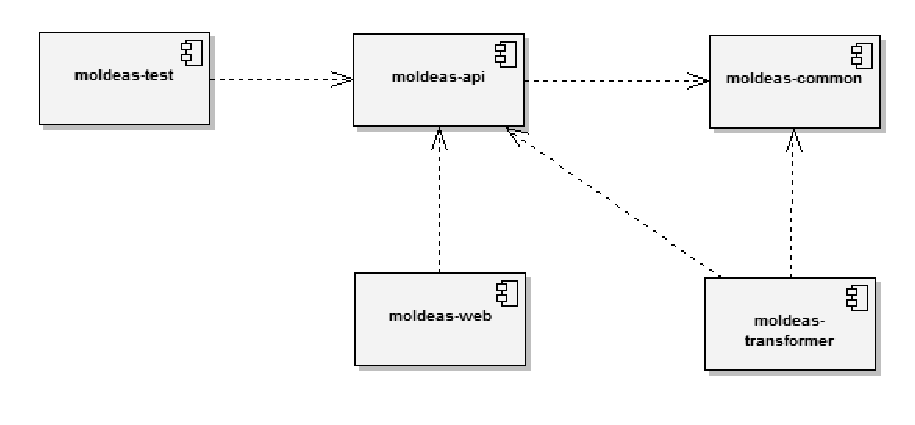
\includegraphics[width=12cm]{images/phd/moldeas/moldeas-componentes}
\caption{Componentes del sistema MOLDEAS.}
\label{fig:moldeas-components}
\end{figure}

\subsection{Arquitectura de alto nivel}
%Diagramas de componentes, diagramas de paquetes
El despliegue de una infraestructura de datos enlazados requiere la cooperación de diferentes elementos 
\textit{hardware} y \textit{software}. Según el análisis realizado de cada uno de los componentes un diagrama 
de despliegue de la arquitectura propuesta en MOLDEAS se presenta en la Figura~\ref{fig:moldeas-despliegue}. 
La descripción de cada uno de estos nodos y componentes es la siguiente:

\begin{itemize}

\item Nodo web. En el cual se encuentran disponibles un servidor web \gls{HTTP} como es Apache2 HTTP Server, este elemento \textit{software} sirve como punto 
de entrada a los elementos del sistema, tanto para el consumo de datos enlazados directamente por otras máquinas como para las peticiones 
relativas al componente \textit{moldeas-web}. También, se utiliza este servicio para albergar una aplicación 
de ejecución de consultas \textit{on-line} en SPARQL como \gls{SNORQL}, sin necesidad de utilizar directamente 
el interfaz propuesto por el \textit{endpoint} de SPARQL.

\item Nodo de aplicaciones web. En el cual se encuentra instalado un contenedor de aplicaciones web \gls{J2EE} como Apache Tomcat, 
con el objetivo de albergar las aplicaciones relativas al \linkeddata \textit{frontend} y a la aplicación \textit{moldeas-web}. 

\item Nodo repositorio RDF. En el cual se instala el repositorio \gls{RDF}, en el cual se almacenan y publican 
los datos enlazados provenientes de los anuncios de licitación. La publicación de datos enlazados se realiza a través de su almacenamiento 
en un repositorio RDF nativo como Virtuoso de OpenLink, suministrando adicionalmente un \textit{endpoint} SPARQL para que los 
datos puedan ser reutilizados y consumidos tanto por la propia aplicación de \textit{moldeas-api} como por clientes 
de forma externa, en este caso se por el \linkeddata \textit{frontend} y SNORQL.

\end{itemize}

Físicamente estos nodos y componentes se han diseñado de forma separada ya que la comunicación entre los mismos 
se realiza mediante delegación de consultas y comunicación mediante HTTP. De esta manera, se permite que el sistema 
sea escalable y flexible, pudiendo sustituir el entorno tecnológico seleccionado por otros proveedores.

Los componentes especificados en MOLDEAS tienen un doble carácter ya que algunos son utilizados de forma \textit{off-line} como 
es el caso de \texttt{moldeas-transformer} y \texttt{moldeas-test}, específicamente para los procesos de producción y validación 
de datos enlazados, mientras que otros como \textit{moldeas-web} sirven como cliente de los servicios proporcionados 
en \texttt{moldeas-api} de forma \texttt{on-line}. Transversalmente \textit{moldeas-common} se utiliza a lo largo de cualquier 
ejecución ya que contiene las clases \textit{Helper} necesarias para la ejecución de tareas comunes.

\begin{figure}[!htb]
\centering
	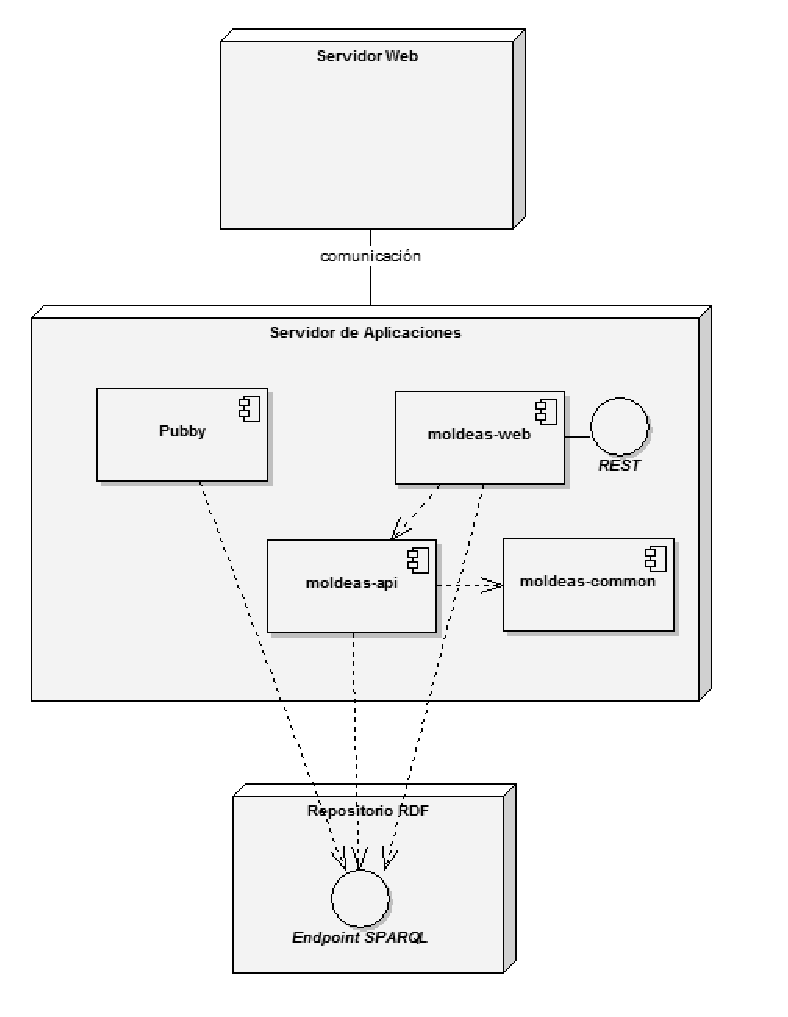
\includegraphics[width=12cm]{images/phd/moldeas/moldeas-despliegue}
\caption{Diagrama de Despliegue de MOLDEAS.}
\label{fig:moldeas-despliegue}
\end{figure}

\subsection{Entorno Tecnológico}
En el momento de analizar y diseñar un conjunto de componentes \textit{software} es necesario seleccionar aquellas 
bibliotecas y herramientas que suministren determinadas funcionalidades de base. La selección estratégica 
de esta tecnología y herramientas se describe someramente a continuación:

\begin{itemize}
 \item Lenguaje de programación Java 1.6. En el campo de la Web Semántica y en particular de la iniciativa de 
datos enlazados, la mayoría de las bibliotecas y funcionalidades externas se encuentran programadas 
en este lenguaje, por lo que unido a la experiencia propia del autor la decisión de uso de este lenguaje 
queda perfectamente justificada.
\item Apache Maven2. El desarrollo de aplicaciones debe realizarse de forma sostenible, es por ello que esta herramienta da 
soporte a todo el proceso de construcción de software: compilación, pruebas, empaquetado, despliegue, documentación, ejecución, etc. 
Además de proveer los mecanismos apropiados para la gestión de dependencias de forma declarativa. 
\item Eclipse \gls{IDE}. La edición del código fuente de las clases Java se ha realizado a través de este entorno de desarrollo, ampliamente 
asentado en la comunidad Java y con una excelente comunidad que proporciona herramientas extra a través de distintos 
\textit{plugins}, proporcionando un entorno productivo y con altas capacidades para el desarrollador. Adicionalmente, Maven 
es capaz de generar a través de su fichero de configuración la estructura de un  proyecto de Eclipse de forma automática.
\item Repositorio de código fuente. Se ha seleccionado la forja de proyectos de Google Code para albergar los cambios y las actualizaciones 
maduras a través del sistema de control de versiones Mercurial.
\item Jena 2.6.4. Biblioteca Java de base tecnológica para la Web Semántica que incluye las principales funciones para el tratamiento de \gls{RDF}, \gls{OWL}, etc. 
así como facilita la ejecución de consultas \gls{SPARQL} tanto de forma local (en memoria) como distribuida (en un \textit{endpoint}).
\item Log4j 1.2.14. Biblioteca Java para la gestión del sistema de registro de una aplicación mediante la cual se puede especificar 
los distintos niveles de registro así como la serialización de los mismos.
\item Junit 4.0. \textit{Framework} Java para la ejecución de pruebas unitarias con un amplio abanico de configuraciones y extras 
para el diseño de pruebas de integración, regresión, etc.
\item Apache \gls{Lucene} 2.9.0. Motor de búsqueda sintáctica en Java con amplias posibilidades tanto para el indexado de documentos, procesamiento 
de lenguaje natural y ejecución de consultas.
\item Apache \gls{Solr} 1.4.1. Plataforma empresarial de búsqueda en Java basada en Apache Lucene que añade nuevas funcionales como nuevos 
filtros para el procesamiento de lenguaje natural.
\item Apache \gls{Mahout} 0.4. Biblioteca Java con un amplio espectro de algoritmos de \textit{data mining} y aprendizaje automático, con capacidades 
para integrarse con otras herramientas como Apache Hadoop y que propone un framework extensible para la creación de nuevos algoritmos.
\item Spring 2.5. \textit{Framework} Java para la creación de aplicaciones empresariales basado en la técnica inversión de control y el uso 
de \textit{Plain Old Java Object} (\gls{POJO}s) para el diseño flexible y el desarrollo ágil de \textit{software}.
\item Jersey \gls{REST} 0.8. Biblioteca Java para la creación de servicios web REST mediante anotaciones.
\item Jquery 1.4.1. \textit{Framework} para el desarrollo de interfaces de usuario enriquecidos basados en HTML+CSS+Javascript.
\item Exhibit 2.2.0. Biblioteca basada en Javascript para el desarrollo de interfaces con múltiples vistas para la presentación 
de datos en general.
\item \gls{Pubby} 0.3.3. \linkeddata \textit{frontend} para la negociación de contenido y presentación de datos enlazados disponibles 
a través de un \textit{endpoint} de \gls{SPARQL}.
\item \gls{SNORQL}. Aplicación basada en HTML+Javascript para la realización de consultas \textit{on-line} sobre \textit{endpoints} de SPARQL.

\end{itemize}




















\section{Consideraciones Generales de Diseño}
En un sentido amplio, dado un problema y un dispositivo en el cual resolverlo, es necesario suministrar un método preciso de respuesta a la casuística 
planteada en el problema de acuerdo al dispositivo objetivo, a tal método se denomina \textit{algoritmo}. El diseño de algoritmos\cite{Vallecillo} 
tiene dos componentes importantes:

\begin{enumerate}
  \item El primero se refiere a la búsqueda de métodos o procedimientos, secuencias
finitas de instrucciones adecuadas al dispositivo del cual se dispone, que permita resolver el problema.  
\item  El segundo permite medir de alguna forma el coste (en tiempo y recursos) de consumo de un algoritmo con el fin de encontrar la
solución, ofreciendo la posibilidad de comparar distintos algoritmos que resuelven un mismo problema.
\end{enumerate}

Una vez que se dispone de un algoritmo que funciona correctamente, es necesario
definir criterios con el objetivo de medir su rendimiento o comportamiento. Estos criterios se centran principalmente en su 
simplicidad y en el uso eficiente de los recursos. La sencillez es una característica sensiblemente interesante en el diseño 
de algoritmos, facilitando su verificación, el estudio de su eficiencia y el mantenimiento. De ahí que muchas veces se priorice la simplicidad y legibilidad 
del código frente a alternativas más crípticas y eficientes del algoritmo. Por otra parte, el uso eficiente de los recursos suele medirse en función de dos
parámetros: el \textit{espacio}, es decir, memoria utilizada, y el \textit{tiempo}, unidades de tiempo de ejecución. En ambos casos, 
se hace referencia a los costes que supone la búsqueda de la solución al problema planteado mediante un algoritmo, además estos dos parámetros 
son utilizados para una posible comparación ulterior de los algoritmos entre sí.

El tiempo de ejecución de un algoritmo dependerá de diversos factores como los datos de entrada que le suministremos, la calidad del código
generado por el compilador para crear el programa objeto, la naturaleza y rapidez de las instrucciones máquina del procesador concreto que ejecute el programa, y la
complejidad intrínseca del algoritmo.  Existen dos tipos posibles de estudio sobre el tiempo:

\begin{enumerate}
\item  Áquel que proporciona una medida teórica (a priori), consistiendo en la obtención de una función que acote 
(inferior o superiormente) el tiempo de ejecución del algoritmo para unos valores de entrada determinados.
\item  El qué ofrece una medida real (a posteriori), consistiendo la medición del tiempo de ejecución del algoritmo para unos valores de entrada determinados 
y un entorno de ejecución particular.
\end{enumerate}

Ambas medidas son importantes puesto que si bien la primera nos ofrece estimaciones
del comportamiento de los algoritmos de forma independiente del ordenador en donde serán implementados y sin necesidad de ejecutarlos, 
la segunda representa las medidas reales del comportamiento del algoritmo. 

\subsection{Consideraciones Diseño de Programas}\label{consideraciones-diseno}
El objetivo de implementación del sistema \gls{MOLDEAS} recae en suministrar parcialmente soporte 
a los distintos procesos implicados en el ciclo de vida de datos enlazados, 
si bien algunas tareas se realizan mediante el uso de ciertas herramientas, existen otras que deben ser parametrizadas e implementadas 
para ofrecer un entorno homogéneo para el manejo de la información y datos 
provenientes de los anuncios de licitación. La separación de responsabilidades 
entre los distintos componentes se realiza de acuerdo a su funcionalidad, de esta manera 
es posible realizar cambios transparentes en los componentes sin que los otros sean 
involucrados en el proceso de cambio: implementación, prueba y empaquetamiento. Por ello, 
se han definido los interfaces de comunicación entre los mismos como un API para que 
cualquier futuro desarrollo se apoye en este \textit{framework} para añadir nuevas 
funcionalidades. Las claves para un diseño abierto de un \gls{API} 
coinciden en muchos sentidos con los de un lenguaje de programación \cite{Interpretes}:

\begin{description}
\item[Concisión notacional:] el API deberá proporcionar un entorno con un nivel
de detalle adecuado: interfaces claras, simples, unificadas etc. Las posibles 
ampliaciones sobre el \textit{framework} de \textit{MOLDEAS} deben resultar sencillas
y no presentar inconvenientes para el programador comprender y extender su diseño.

\item[Ortogonalidad:] la funcionalidad del API debe suministrar el mecanismo
adecuado para combinar nuevos componentes y rechazar algunos de los ya
presentes. Por ejemplo la adición de nuevas restricciones no debe suponer una
recodificación del código del algoritmo.

\item[Abstracción:] el diseño del API debe basarse en el uso de técnicas como
los patrones de diseño e interfaces favoreciendo la abstracción de algoritmos.

\item[Seguridad:] los algoritmos implementados debe tener puntos obligatorios de restricciones
para verificar por ejemplo su terminación aunque se añadan nuevas
restricciones. 

\item[Expresividad:] el API debe ser lo suficientemente ``rica'' como para que
nuevas ampliaciones puedan ser formuladas de forma sencilla de acuerdo a la información 
y datos presentes en los anuncios de licitación y en su modelo formal. 

\item[Extensiblidad:] el API debe basarse en técnicas de programación que
favorezcan la adición de nuevas características y su adaptación para nuevas
configuraciones del algoritmo


\item[Portabilidad:] el lenguaje seleccionado para proporcionar estas técnicas
debe poseer esta característica.

\item[Eficiencia:] en cualquier implementación de un algoritmo o conjunto de los mismos esta característica es fundamental y
aunque el API diseñado, atendiendo a las características anteriores pueda
sobrecargar la ejecución básica de los procesos, su penalización en tiempo no es tan alta 
como para descartar los principios de diseño anteriores.

\item[Librerías e interacción con el exterior:] la ejecución de las funcionalidades 
provistas deberá ser independiente del lenguaje de ontologías utilizado, así aislamos el
conjunto de técnicas de la fuente de conocimiento favoreciendo el uso del
cualquier lenguaje de formalización.

\item[Entorno:] para facilitar la depuración de los algoritmos realizados se
proveerá un entorno gráfico en el cual poder visualizar la ejecución.
\end{description}

Además de estas principios generales para el diseño del API, hay que tener en
cuenta: 

\begin{itemize}
  \item El entorno de ejecución puede ser una aplicación web, por lo que, se
  deberá tener en cuenta en el diseño para que pueda fácilmente integrarse con
  \textit{frameworks} como Spring.
  \item La mayoría de las aplicaciones utilizando Web Semántica utilizan el
  lenguaje Java, por lo tanto, este será el lenguaje seleccionado en su última versión.
\end{itemize}
 
\subsection{Patrones de Diseño}\label{patrones}
Con el objetivo de cumplir los criterios antes mencionadas, el sistema \gls{MOLDEAS} se basará en la aplicación 
intensiva de patrones de diseño\cite{Gamma,CoreJ2EEPatterns} como buena práctica 
de programación. Normalmente estos patrones indican la interacción que ha de realizarse entre los distintos elementos 
que participan en el problema. De esta manera para cada problema tendremos un 
conjunto de objetos, cada uno de los cuales realizará una función proveyendo servicios a 
los demás objetos implicados. Los patrones de diseño proponen soluciones con distintas características: 
elegantes, modulares, escalables y flexibles. Una posible definición de los mismos 
se presenta a continuación:

\begin{Frame}
Los patrones de diseño representan soluciones para problemas recurrentes en la ingeniería del \textit{software}.
\end{Frame}

En general, se trata de soluciones estándar para un problema habitual en programación que utiliza 
distintas técnicas para la flexibilización del código intentando al mismo tiempo satisfacer 
ciertos criterios no funcionales. Se suelen asimilar a una estructura determinada de implementación 
que cumple una finalidad determinada y permite describir ciertos aspectos de un programa.

No obstante, pese a que los patrones nos ofrecen buenas soluciones puede darse el caso de que 
resulte contraproducente el uso de los mismos. El uso de estas técnicas debe realizarse, 
por tanto, en el momento justo. La problemática reside en establecer cuándo su aplicación 
es adecuada y se pueden citar varios criterios:
\begin{itemize}
    \item El código del programa ha crecido exponencialmente.
    \item Las clases de un programa aglutinan código semánticamente no corresponde con su funcionalidad.
    \item Se deben realizar pruebas unitarias de clases.
    \item El diseño del programa es altamente complejo y las relaciones entre las distintas 
clases es opaca.
   \item La comunicación con otros desarrolladores ha decaído debido a la complejidad del código.
\end{itemize}

El libro \textit{The Ganf of Four(Gof)}~\cite{Gamma} fue el pionero en introducir estas técnicas de 
programación caracterizando las mimas en tres niveles:
\begin{description}
    \item [Patrones creacionales:]se utilizan para la creación, inicialización
    Podemos destacar: \textit{Abstract Factory}, \textit{Builder}, \textit{Factory Method}, \textit{Prototype} o
    \textit{Singleton}.
    \item [Patrones estructurales:]su objetivo es separar la interfaz de
    operaciones de la implementación. Tratan de organizar cómo las clases y
    objetos se agrupan para generar estructuras y organizaciones más grandes.
    Por ejemplo: \textit{Adapter}, \textit{Bridge}, \textit{Composite}, \textit{Decorator} o \textit{Facade}.
    \item [Patrones de comportamiento:] describen la comunicación entre los
    objetos.  \textit{Chain of Responsability}, \textit{Command}, \textit{State}, \textit{Strategy} o \textit{Visitor} son
    ejemplos de este conjunto.
\end{description}

En combinación con los patrones de diseño, se encuentra la técnica de \textit{refactoring}~\cite{Fowler1999}, 
utilizada para reestructurar y refinar el código fuente (en muchos casos aplicando un determinado patrón) 
sin alterar la funcionalidad o comportamiento externo del mismo.




\section{Diseño de Componentes del Sistema MOLDEAS}
\input{chapters/moldeas/disenyo-componentes}
\section{Pruebas del Sistema MOLDEAS}\label{sect:pruebas-moldeas}
\input{chapters/moldeas/pruebas-componentes}
\section{Utilizando el Sistema MOLDEAS}
\input{chapters/moldeas/uso-moldeas}
